\section{Finite Dimensional Projective Unitary Representations}
\subsection{Motivation}
So far, we have only been dealing with ordinary representations of Lie groups and Lie algebras. We now introduce the other class of representations: projective unitary representations.

Let $V$ be a finite dimensional state space. We are often interested in unitary operators on $V$. We can go one step further. Recall that two vectors in the state space that differ by multiplication by a constant are considered to represent the same physical state. Thus we are also interested in the projective unitary group, which we define as
\[
    \frac{U(V)}{\{e^{i\theta}I\}} = \PU(V).
\]
A projective unitary representation is a map $\Pi: G \rightarrow \PU(V)$. We will see that this concept is useful when studying spin.

\subsection{Definitions}
Many of the concepts of ordinary representations carry over to projective unitary representations.
\begin{itemize}
    \item An projective unitary representation $\Pi$ is irreducible if the only invariant subspaces of $V$ under all $U$ such that $[U] \in \Pi(G)$ are $0$ and $V$.
    \item A projective unitary Lie algebra representation is a homomorphism $\mathfrak\pi: g \rightarrow \pu(V)$, where $\pu(V)$ is the Lie algebra corresponding to $\PU(V)$.
    \item A projective unitary representation $\pi$ is irreducible if the only invariant subspaces under $U$ for every $[U] \in \pi(G)$ are $0$ and $V$.
\end{itemize}

\subsection{Two Lemmas On De-Projectivization}
We now state a few technical results we will need when studying spin.

Given an representation $\Sigma: G \rightarrow \U(V)$, we can get a projective unitary representation $\Pi: G \rightarrow \PU(V)$ by composing with the natural map $Q: \U(V) \rightarrow \PU(V)$. We can ask the converse: can we de-projectivize each $\Pi: G \rightarrow \PU(V)$ into a map $\Sigma: G \rightarrow \U(V)$? This is generally not possible. However, we can de-projectivize at the Lie algebra level:
\begin{figure}[H]
    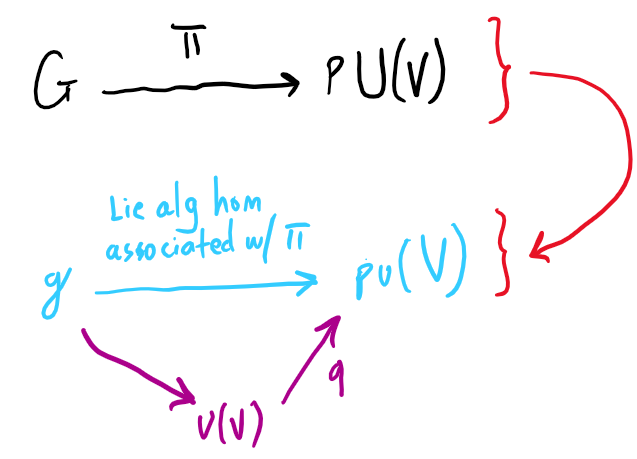
\includegraphics[width=0.5\textwidth]{figures/de-projectivization}
    \centering
\end{figure}

Here, $q: \uu(v) \rightarrow \pu(v)$ is the Lie algebra homormorphism associated with $Q$.

We can also de-projectivize at the expense of passing from $G$ to the universal cover $G^*$.
\begin{figure}[H]
    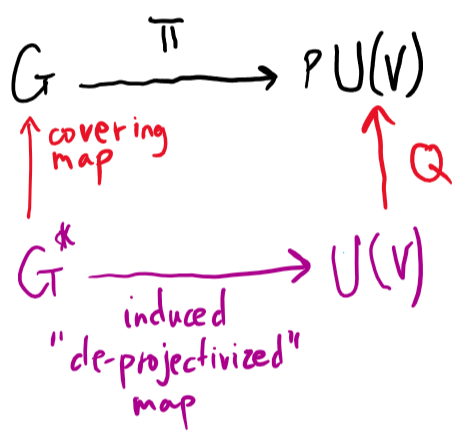
\includegraphics[width=0.4\textwidth]{figures/de-projectivization2}
    \centering
\end{figure}

\subsection{Inifinite Dimensional Projective Unitary Representations}
Like ordinary representations, we can allow $V$ to be infinite dimensional if we add extra technical conditions to our definition of projective unitary representations.
